\section{动土开工}

将前面的各种东西准备好后,就可以正式开始一个项目了。这里还需要强调一点,我们文件的结构方式,一个项目文件夹下包含四个子文件夹。例如本篇文章的目录结构情况如图 \ref{fig:screenshot002} 。其中 \lstinline|1| 放子文件,date 当参考文献和其它,picture 放图片,picture 下放位图,svg里面放矢量图片,table下放表格文件。 
% TODO: \usepackage{graphicx} required
\begin{figure}[h!]
	\centering
	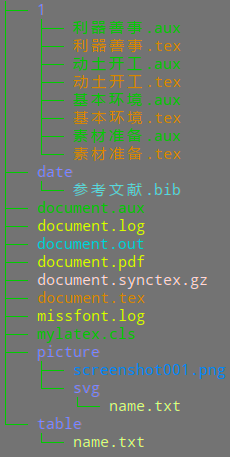
\includegraphics[width=0.2\linewidth]{picture/screenshot002}
	\caption{文档结构}
	\label{fig:screenshot002}
\end{figure}

其中svg和table两个目录下的 name.tex 文件,是名称存放文件,可用如下命令批量生成
\begin{lstlisting}[language=bash]
seq -f "name-%04g" 1 9999 > name.txt
\end{lstlisting}
各个脚本在编写过程中也是按照如此目录设计,若需改动目录结构,请将脚本中的目录一同改动。


至此,即可。Happy \LaTeX !




